\section{Allgemeine Beschreibung}
\label{sec:generalProvision}
%\note{In diesem Kapitel sollen Hintergrundinformationen gegeben werden, keine spezifischen Anforderungen. Diese folgen im nächsten Kapitel. In diesem Kapitel muss genau geklärt werden, was zum System gehört und was nicht, d.h. die Systemgrenze muss hier zwingend festgelegt werden.}


\subsection{Systemübersicht}
\begin{figure}[!h]
	\centering
	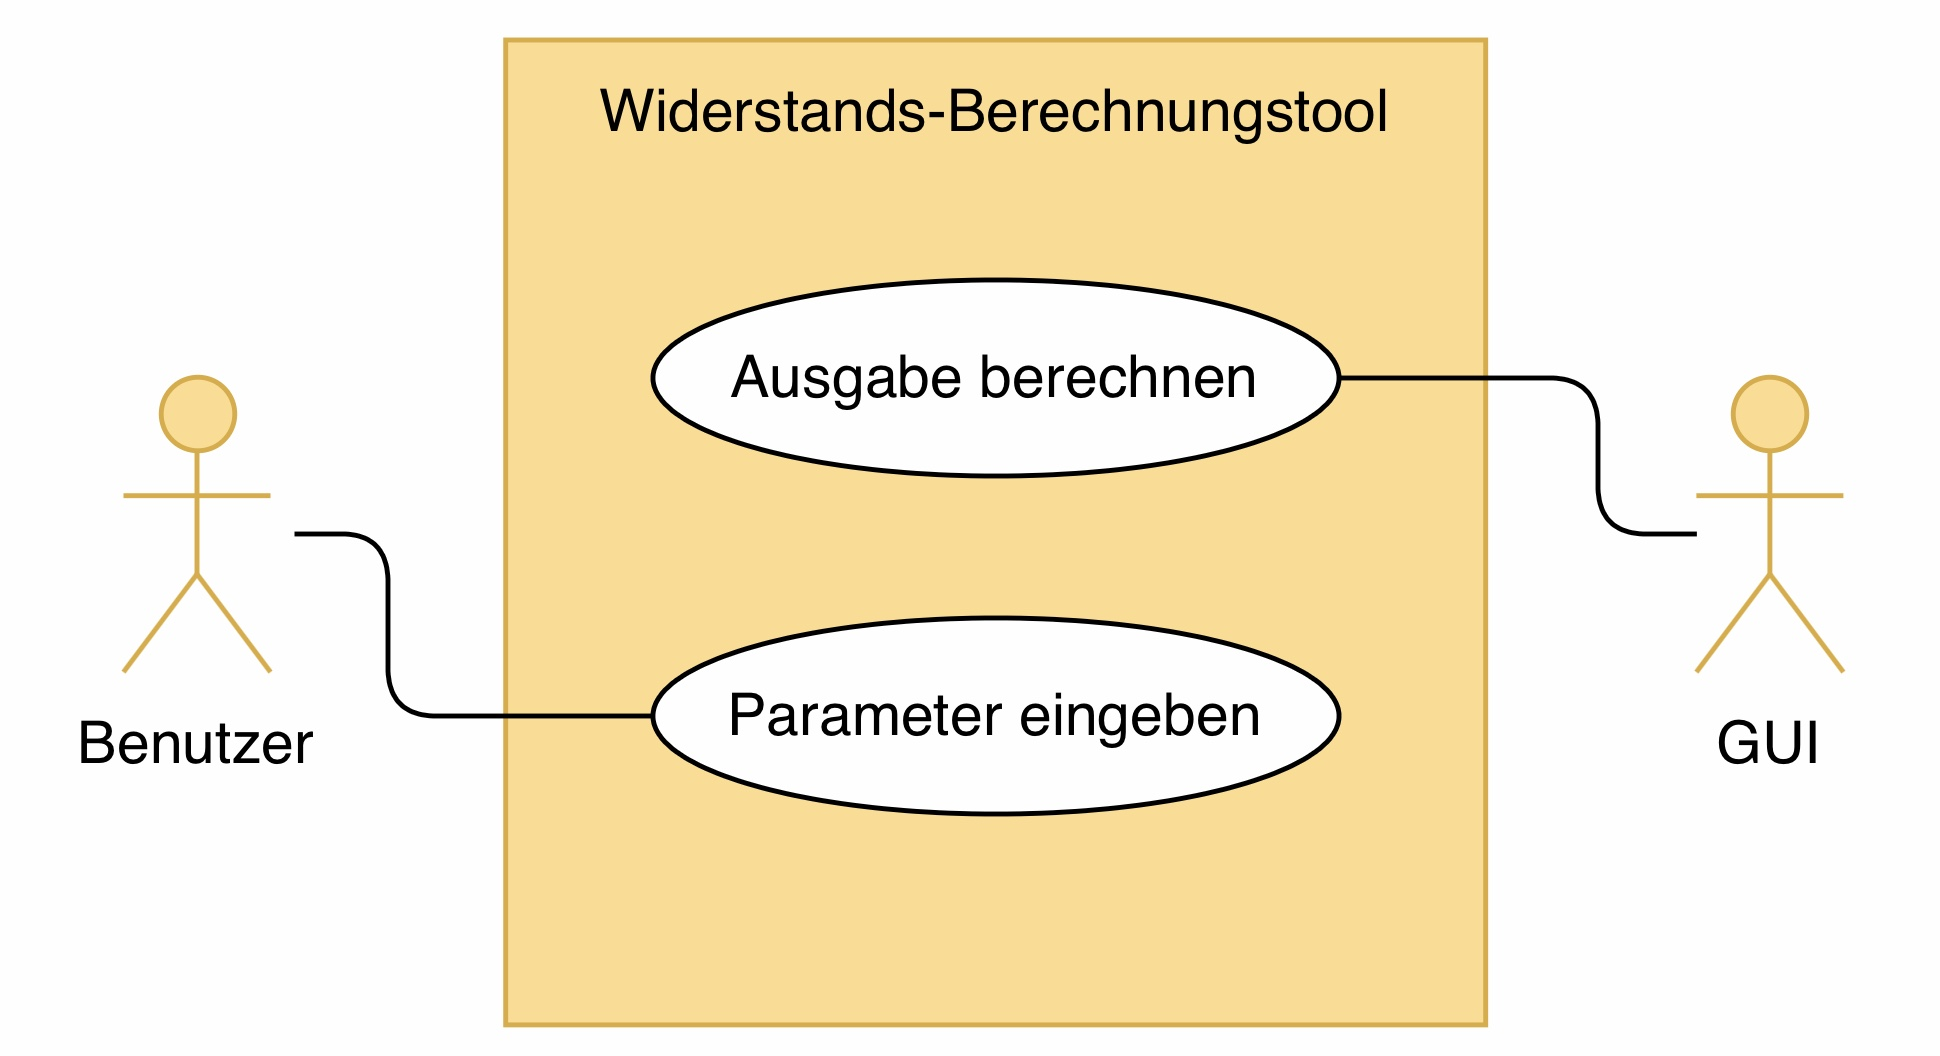
\includegraphics[width=11cm]{./images/Use-Case.jpg}
	\caption{Kontextdiagramm (Festlegung der Systemgrenze)}
	\label{fig:contextDiagram}
\end{figure}
Das Tool verfügt über ein GUI mit Eingabefeld, in welches der User die Parameter des gewünschten Spannungsteilers eingibt. Nach erfolgter Berechnung gibt das Tool über das GUI die Widerstandswerte zurück, welche den vorgegebenen Parametern am ehesten entsprechen.

%\note{Definieren Sie das Umfeld des Systems mit den Schnittstellen des Systems zu seinem Umfeld und das System selbst. Hier muss die Systemgrenze in Form eines Kontextdiagramms gezogen werden. Aus diesem Abschnitt muss eindeutig hervorgehen, was innerhalb der Systemgrenze liegt (was mZuss entwickelt werden?) und was ausserhalb.}


%\note{This subsection should also describe how the system operates inside various constraints. For example, these constraints could include
%\begin{enumerate}
%\item System interfaces
%\item User interfaces
%\item Hardware interfaces
%\item Software interfaces
%\item Communications interfaces
%\item Memory
%\item Operations
%\item Site adaptation requirements
%\end{enumerate}
%}

\subsection{Produktfunktionen}
Berechnen der beiden Widerstandswerte aus der gewünschten E-Reihe.
%\note{Hier soll eine \textbf{Zusammenfassung} der Hauptfunktionen angeboten werden, welche das System erfüllen soll.}

\subsection{Benutzereigenschaften}
Jeder Benutzer mit wenig technischem Hintergrund soll das Gerät verwenden können.
%\note{Festlegung der Benutzer (Benutzergruppen), welche mit dem System arbeiten sollen, z.B. Routinebenutzer, Servicetechniker, Administrator. Dazu gehört auch die Definition der Kenntnisse und Erfahrungen der einzelnen Gruppen. Falls die funktionalen An-forderungen mittels Use Case – Diagrammen formuliert werden, dann entspricht dies den Actors, welche Personen repräsentieren.}

\subsection{Einschränkungen}
Keine
%\note{This subsection of the SRS should provide a general description of any other items that will limit the developer's options. These include:

%\begin{enumerate}
%\item Regulatory policies
%\item Hardware limitations (e.g., signal timing requirements)
%\item Interfaces to other applications
%\item Parallel operation
%\item Audit functions
%\item Control functions
%\item Higher-order language requirements
%\item Signal handshake protocols (e.g., XON-XOFF, ACK-NACK)
%\item Reliability requirements
%\item Criticality of the application
%\item Safety and security considerations
%\end{enumerate}}

\subsection{Annahmen und Abhängigkeiten}
Keine
%\note{This subsection of the SRS should list each of the factors that affect the requirements stated in the SRS. These factors are not design constraints on the system but are, rather, any changes to them that can affect the requirements in the SRS. For example, an assumption may be that a specific operating system will be available on the hardware designated for the software product. If, in fact, the operating system is not available, the SRS would then have to change accordingly.}

\subsection{Priorisierung der Anforderungen}
Keine
%\note{Falls die Anforderungen unterschiedliche Prioritäten haben, bzw. einzelne Anforderungen erst in einer späteren Version implementiert werden sollen, dann kann das hier aufgelistet werden, z.B.
%\begin{itemize}
%\item Muss-Anforderung: dies ist eine Anforderung, welche für das System essentiell und unabdingbar ist, bzw. das System würde keinen Sinn ergeben, wenn diese Anforderung nicht implementiert wäre.
%\item Soll-Anforderung: eine Soll-Anforderung ist nicht unabdingbar, trägt jedoch zur wesentlichen Verbesserung des Systems bei. Sie soll wenn möglich realisiert werden.
%\item Wunsch-Anforderung (nice to have): diese Anforderung trägt zur Verbesserung des Systems bei, ist jedoch nicht unbedingt notwendig. Es ist ein Plus wenn diese Anforderung realisiert werden kann.
%\end{itemize}

